%%%%%%%%%%%%%%%%%%%%%%%%%%%%%%%%%%%%%%%%%%
% Engineering problems / LaTeX Template
%		Semester 6
%		Institut d'Optique Graduate School
%%%%%%%%%%%%%%%%%%%%%%%%%%%%%%%%%%%%%%%%%%
%	6N-IntNum-BlocRobot	/ Embedded System
%%%%%%%%%%%%%%%%%%%%%%%%%%%%%%%%%%%%%%%%%%
%
% Created by:
%	Julien VILLEMEJANE - 19/oct/2024	
%
%%%%%%%%%%%%%%%%%%%%%%%%%%%%%%%%%%%%%%%%%%
% Professional Newsletter Template
% LaTeX Template
% Version 1.0 (09/03/14)
%
% Created by:
% Bob Kerstetter (https://www.tug.org/texshowcase/) and extensively modified by:
% Vel (vel@latextemplates.com)
% 
% This template has been downloaded from:
% http://www.LaTeXTemplates.com
%
% License:
% CC BY-NC-SA 3.0 (http://creativecommons.org/licenses/by-nc-sa/3.0/)
%
%%%%%%%%%%%%%%%%%%%%%%%%%%%%%%%%%%%%%%%%%

\documentclass[a4paper,11pt,titlepage]{article} % The default font size is 10pt; 11pt and 12pt are alternatives

%%%%%%%%%%%%%%%%%%%%%%%%%%%%%%%%%%%%%%%%%%%%%%%%%%%%%%%%%%%%%%%%%%%%%%%%%%%%%%%%%%%%%%%%%%%%%%%%%%%%%%%%%%%%%%%%%%%%%%%%%%%%%%%%%%%%%%%%%%%%%%%%%%%%%%%%%%%%%%%%%%%%%%%%%%%%%%%%%%%%%%%%%%%%%%%%%%%%%%%%%%%%%%%%%%%%%%%%%%%%%%%%%%%%%%%%%%%%%%%%%%%%%%%%%%%%
\usepackage{opto_elec_villemejane}

%%%%%%%%%%%%%%%%%%%%%%%%%%%%%%%%%%%%%%%%%%%%%%%%
%%%%%%%%%%%%%%%%%%%%%%%%%%%%%%%%%%%%%%%%%%%%%%%%
\begin{document}



% Page de garde
\begin{titlepage}

\begin{center}
	\begin{minipage}{2.5cm}
	\begin{center}
		
\includegraphics[width=8cm]{images/Logo-LEnsE.png}
	\end{center}
\end{minipage}\hfill
\begin{minipage}{10cm}
	\begin{center}
	\textbf{Institut d'Optique Graduate School }\\[0.1cm]
    \textbf{Interfaçage Numérique}


	\end{center}
\end{minipage}\hfill


\vspace{4cm}


{\huge \bfseries \textsc{Interfaçage Numérique}} \\[0.5cm]
{\large \bfseries Travaux Pratiques} \\[0.2cm]
Semestre 6

\vspace{2cm}
% Title
\rule{\linewidth}{0.3mm} \\[0.4cm]
{ \huge \bfseries\color{violet_iogs} Robotique et systèmes embarqués\\[0.4cm] }
\rule{\linewidth}{0.3mm} \\[1cm]

4 séances

\bigskip

\begin{center}
	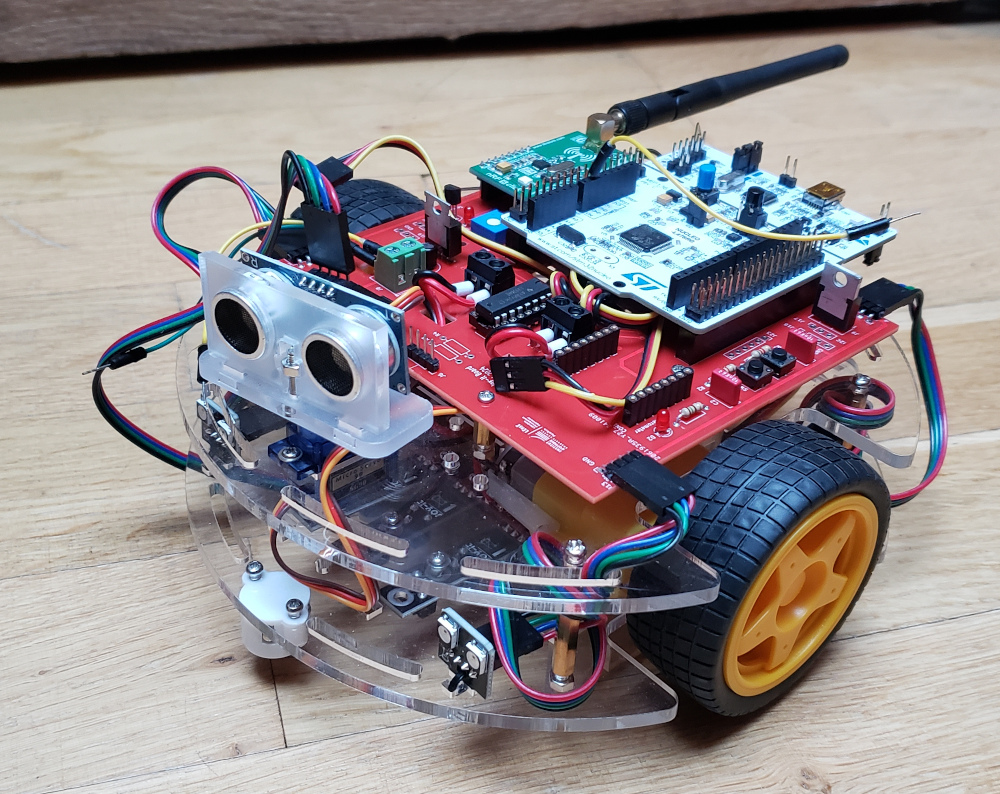
\includegraphics[width=0.4\textwidth]{images/robot_joycar.jpg}
\end{center}

\vfill

\textit{Ce sujet est disponible au format électronique sur le site du LEnsE - https://lense.institutoptique.fr/ dans la rubrique Année / Première Année / Interfaçage Numérique S6 / Bloc 1 Systèmes embarqués / Robotique.}

% Bottom of the page
%{\textbf{\large {Année universitaire} 2024-2025}}

\end{center}
\end{titlepage}

\newpage
\strut % empty page


%%%%%%%%%%%%%%%%%%%%%%%%%%%%%%%%%%%%%%%%%%%%%%%%
%%%%%%%%%%%%%    Intro
\newpage
\pagestyle{empty}

\begin{minipage}[c]{.25\linewidth}
	
\includegraphics[width=5cm]{images/Logo-LEnsE.png}
\end{minipage} \hfill
\begin{minipage}[c]{.4\linewidth}

\begin{center}
\vspace{0.3cm}
{\Large \textsc{Interfaçage Numérique}}

\medskip

6N-047-SCI \qquad \textbf{\Large Bloc Robot}

\end{center}
\end{minipage}\hfill

\vspace{0.5cm}

\noindent \rule{\linewidth}{1pt}

{\noindent\Large  \rule[-7pt]{0pt}{30pt} \textbf{Robotique et systèmes embarqués}}

\noindent \rule{\linewidth}{1pt}

\bigskip 

%%%%%%%%%%%%%%%%%%%%%%%%%%%%%%%%%%%%%%%%%%%%%%%%
%%%%%%%%%%%%%    A A V

{\large À l'issue des séances de TP concernant le \textbf{bloc de robotique}, les étudiant$\cdot$es seront capables de :}

\medskip

\begin{itemize}
	\item Développer et mettre en \oe{}uvre une \textbf{solution d'électronique embarquée} pour \textbf{mettre en mouvement un robot}
	\item Concevoir un \textbf{programme embarqué} permettant de \textbf{rendre autonome les mouvements d'un robot}
\end{itemize}

\noindent \rule{\linewidth}{1pt}


%%%%%%%%%%%%%%%%%%%%%%%%%%%%%%%%%%%%%%%%%%%%%%%%
%%%%%%%%%%%%%    Objectifs

\section{Objectifs du mini-projet}

L'objectif principal de ce mini-projet est de \textbf{développer le code embarqué d'une plateforme robotique} lui permettant de se déplacer de manière autonome le long d'une ligne sans percuter d'obstacle.
%	\item soit d'être piloter à distance par une télécommande et d'afficher des informations provenant de capteurs intégrés à la plateforme.  Pour 2025-2026 !!

\begin{center}
	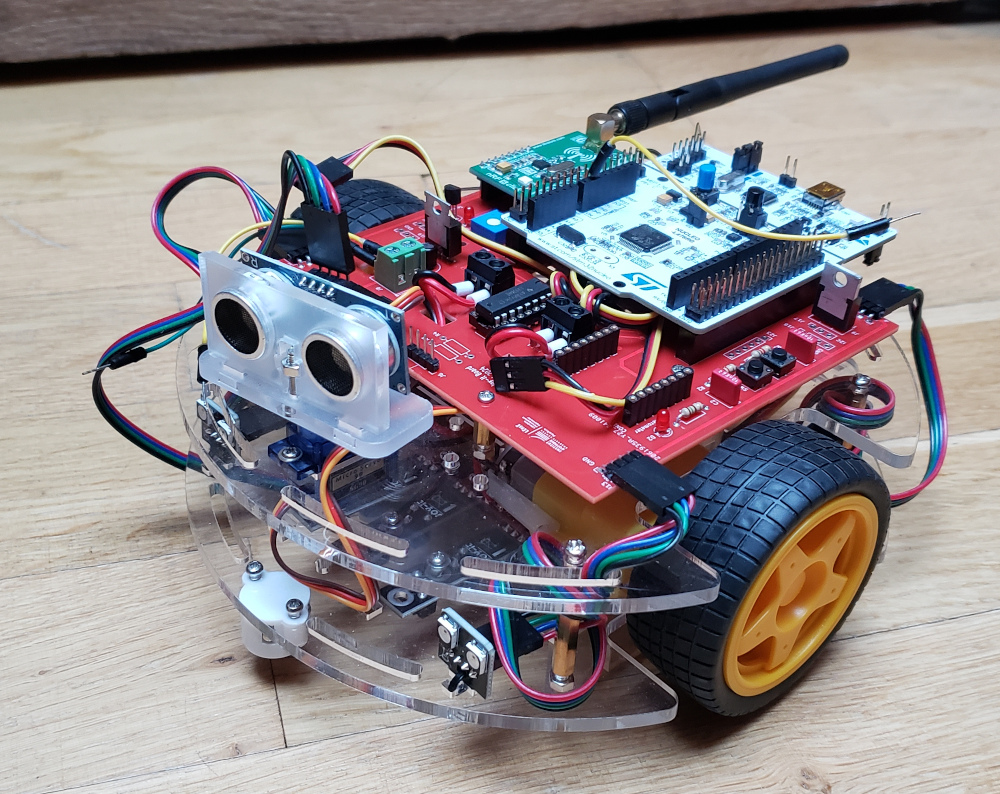
\includegraphics[width=0.4\textwidth]{images/robot_joycar.jpg}
\end{center}


\medskip

Vous aurez à votre disposition une \textbf{maquette} basée sur un robot Joy-It Car. Cette maquette est pilotée par une carte Nucléo (contenant un microcontroleur).


\newpage
%%%%%%%%%%%%%%%%%%%%%%%%%%%%%%%%%%%%%%%%%%%%%%%%
%%%%%%%%%%%%%    Déroulement

\section{Déroulement du bloc}

\textit{La liste des étapes à suivre pour la réalisation du programme embarqué de la plateforme robotique est donnée à titre indicatif. L'ordre et le choix des différentes étapes sont laissés à l'appréciation des différents binômes.}

\textit{Afin de faciliter la réutilisation des codes, il pourra être intéressant de définir des fonctions pour le pilotage des différents éléments.}

\subsection{Séance 1 / MBED et Nucléo-STM32 (sans maquette !!)}

\textit{Le sujet de cette séance est fourni dans un document annexe, disponible aussi sur le site du LEnsE - https://lense.institutoptique.fr/ dans la rubrique Année / Première Année / Interfaçage Numérique S6 / Bloc 1 Systèmes embarqués / Intro MBED et STM32.}

	\begin{description}
		\item[Etape 0 - 30 min] Créer un compte MBED et tester un premier programme
		\item[Etape 1 - 45 min] Piloter des sorties numériques - LED
		\item[Etape 2 - 45 min] Acquérir des données numériques - Bouton-poussoirs
		\item[Etape 3 - 45 min] Mettre en \oe{}uvre des interruptions sur des événements externes
		\item[Etape 4 - 45 min] Utiliser des sorties modulées en largeur d'impulsion (PWM) - LEDs
		\item[Etape 5 - 60 min] Acquérir des données analogiques - Potentiomètre
	\end{description}	


\subsection{Séance 2 / Prise en main de la maquette et déplacements élémentaires}

	\begin{description}
		\item[Etape 6 - 60 min] Piloter l'intensité des LEDs de la maquette
		\item[Etape 7 - 90 min] Piloter les moteurs à courant continu
		\item[Etape 8 - 60 min] Acquérir des données des capteurs de ligne				
		\item[Etape 9 - 60 min] Piloter les phares du robot (NeoPixel)
	\end{description}


\subsection{Séances 3 et 4 - Pilotage de haut niveau}

Les deux séances suivantes seront consacrées au pilotage du robot pour lui permettre de suivre une ligne ou/et d'éviter les obstacles qu'il rencontre sur son chemin.

Les étapes possibles sont les suivantes :

\begin{description}
	\item[Etape 10 - 120 min] Définir et tester une première structure de code permettant de piloter les deux moteurs du robot en fonction de la détection des lignes
	\item[Etape 11 - 90 min] Acquérir les signaux du capteur ultrason
	\item[Etape 12 - 90 min] Piloter le servomoteur associé au capteur ultrason
	\item[Etape 13 - 180 min] Améliorer le programme de contrôle du robot
\end{description}

Vous pourrez également ajouter d'autres éléments présents sur la carte : encodeur de vitesse sur les roues, capteurs de température (analogique ou numérique en I2C), accéléromètre (I2C).



\newpage
\strut % empty page
%%%%%%%%%%%%%%%%%%%%%%%%%%%%%%%%%%%%%%%%%%%%%%%%
%%%%%%%%%%%%%    Séance 2 détaillée
\begin{minipage}[c]{.25\linewidth}
	
\includegraphics[width=4cm]{images/Logo-LEnsE.png}
\end{minipage} \hfill
\begin{minipage}[c]{.4\linewidth}

\begin{center}
\vspace{0.3cm}
{\Large \textsc{Interfaçage Numérique}}

\medskip

6N-047-SCI \qquad \textbf{\Large Bloc Robot}

\end{center}
\end{minipage}\hfill

\vspace{0.5cm}

\noindent \rule{\linewidth}{1pt}

{\noindent\Large \rule[-7pt]{0pt}{30pt} \textbf{Séance 2} / Prise en main de la maquette et déplacements élémentaires} 

\noindent \rule{\linewidth}{1pt}


%%%%%%%%%%%%%%%%%%%%%%%%%%%%%%%%%%%%%%%%%%%%%%%%
%%%%%%%%%%%%%    Objectifs
\section{Objectifs de la séance}

Cette seconde séance est consacrée à la \textbf{prise en main de la maquette} et au développement des \textbf{fonctionnalités permettant les déplacements élémentaires} de la plateforme.


%%%%%%%%%%%%%%%%%%%%%%%%%%%%%%%%%%%%%%%%%%%%%%%%
%%%%%%%%%%%%%    Maquette
\section{Description de la maquette}

\begin{center}
	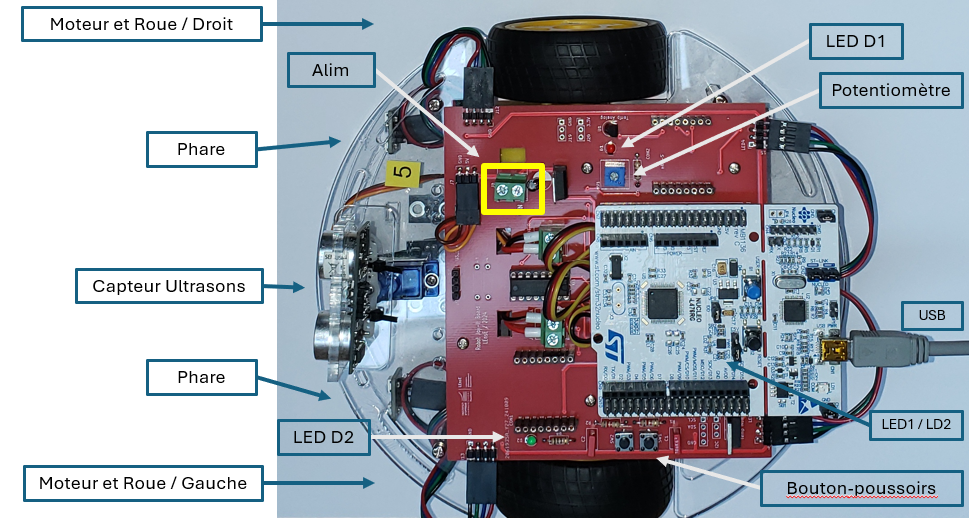
\includegraphics[width=0.8\textwidth]{images/robot_maquette.png}
\end{center}

La maquette est basée sur une plateforme robotique \textbf{Joy-It} \textit{Joy-Car} (\href{https://joy-it.net/en/products/mb-joy-car}{joy-it.net/en/products/mb-joy-car}) constituée :

\begin{itemize}
	\item de \textbf{deux moteurs à courant continu} indépendants, contrôlés par un driver de type L293DN - tension maximale $7\operatorname{V}$ associés à deux encodeurs de position sur les roues motrices ;
	\item de \textbf{trois capteurs de ligne} (en dessous du robot) ;
	\item d'un \textbf{capteur à ultrason} (obstacles) monté sur un servomoteur ;
	\item de \textbf{4 phares}, composés de 2 LEDs RGB de type WS2812 ;
	\item d'une \textbf{carte de contrôle}, composée :
	\begin{itemize}
		\item de deux bouton-poussoirs ;
		\item de deux LEDs standard ;
		\item d'un potentiomètre ;
		\item d'une carte Nucléo L476RG.
	\end{itemize}
\end{itemize}

\textit{Un schéma de la carte et le brochage des différents éléments sont donnés en annexe de ce document.}

\newpage
\subsection{Alimentation électrique}

La plateforme robotique est utilisable dans deux configurations différentes :
\begin{itemize}
	\item \textbf{non-autonome}, reliée en USB, lors de la phase de programmation de la carte de commande ;
	\item \textbf{autonome}, sur batterie ou alimentation externe.
\end{itemize}

\subsubsection{Carte Nucléo}

La carte Nucléo ainsi que la carte de commande (incluant les phares et les capteurs du robot) peut être \textbf{alimentée à l'aide du câble USB} (permettant également la programmation du microcontroleur embarqué sur la carte Nucléo).


\noindent \rule{\linewidth}{1pt}

\textbf{Attention !} Dans ce régime de fonctionnement, les moteurs et servomoteur ne sont pas utilisables (car non alimentés).

\noindent \rule{\linewidth}{1pt}

Le cavalier \textbf{JP5} de la carte Nucléo doit être positionné du côté \textbf{U5V}.

\begin{center}
	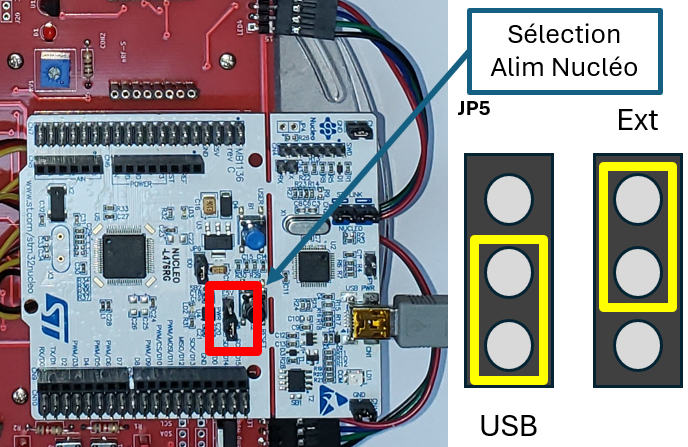
\includegraphics[width=0.5\textwidth]{images/nuc_alim.png}
\end{center}

\textbf{Attention !} Lors de la programmation de la carte Nucléo, il est préconisé de \textbf{ne pas utiliser la partie puissance} !

\subsubsection{Utilisation de la partie puissance (motorisation)}

\noindent \rule{\linewidth}{1pt}

\medskip

\textbf{\large La tension maximale admissible par les moteurs est de $7\operatorname{V}$ !}

\noindent \rule{\linewidth}{1pt}

L'alimentation de cette partie se fait à l'aide du connecteur \textbf{J8}. La broche \textbf{VIN} correspond à la tension positive (comprise entre 5 et 7V) et l'autre broche est reliée à la masse du système.


\noindent \rule{\linewidth}{1pt}

\textbf{Attention !} Il est conseillé de tester la motorisation du robot à l'aide d'une alimentation stabilisée - et surtout protégée en courant ! - avant de passer à l'utilisation totalement autonome sur batterie.


\noindent \rule{\linewidth}{1pt}

\textbf{Attention !} Pour utiliser la partie puissance, il est préconisé de passer la \textbf{carte Nucléo en utilisation autonome} (sur alimentation externe) et ainsi supprimer le lien par le câble USB.

Pour cela, il faut placer le cavalier \textbf{JP5} de la carte Nucléo du côté \textbf{E5V} (E = externe).

\noindent \rule{\linewidth}{1pt}


\newpage
\subsection{Brochage}

\subsubsection{Entrées-Sorties standard}

\begin{center}
\begin{tabular}{|l|l|l|l|}
\hline 
Maquette & \textbf{Broche Nucléo} & Type & Description \\ 
\hline 
\textsc{LED1} & PC7 & Sortie / PWM & Led active à l'\textbf{état bas}\\ 
\textsc{LED2} & PB13 & Sortie / PWM & Led active à l'\textbf{état haut}\\ 
\hline 
\textsc{SW1} & PA11 & Entrée & Bouton-poussoir, par défaut état bas\\ 
\textsc{SW2} & PA12 & Entrée & Bouton-poussoir, par défaut état bas\\ 
\textsc{UserButton} & PC13 & Entrée & Bouton-poussoir, par défaut état haut\\
\hline  
\textsc{POT\_OUT} & PC3 & Entrée analogique & Potentiomètre\\
\hline  
\end{tabular} 
\end{center}

\subsubsection{Moteurs}

\begin{center}
\begin{tabular}{|l|l|l|l|}
\hline 
Maquette & \textbf{Broche Nucléo} & Type & Description \\ 
\hline 
\textsc{MOT\_EN} & PA9 & Sortie & Validation des moteurs\\ 
\hline 
\textsc{MOT\_L\_1} & PB4 & Sortie / PWM & Moteur Gauche direction 1\\ 
\textsc{MOT\_L\_2} & PA8 & Sortie / PWM & Moteur Gauche direction 2\\ 
\hline 
\textsc{MOT\_R\_1} & PA0 & Sortie / PWM & Moteur Droit direction 1\\ 
\textsc{MOT\_R\_2} & PA1 & Sortie / PWM & Moteur Droit direction 2\\ 
\hline  
\end{tabular} 
\end{center}

\subsubsection{Phares NeoPixel / SW2812}

\begin{center}
\begin{tabular}{|l|l|l|l|}
\hline 
Maquette & \textbf{Broche Nucléo} & Type & Description \\ 
\hline 
\textsc{Din\_1} & PC0 & Sortie & Phare avant droit\\ 
\textsc{Din\_2} & PA10 & Sortie & Phare avant gauche\\ 
\textsc{Din\_3} & PC5 & Sortie & Phare arrière gauche\\ 
\textsc{Din\_4} & PA13 & Sortie & Phare arrière droit\\ 
\hline  
\end{tabular} 
\end{center}

\subsubsection{Capteurs}

\begin{center}
\begin{tabular}{|l|l|l|l|}
\hline 
Maquette & \textbf{Broche Nucléo} & Type & Description \\ 
\hline 
\textsc{TEMP\_OUT} & PC2 & Entrée analogique & Capteur de température MCP9700\\ 
\hline 
\textsc{Line\_L} & PA7 & Entrée & Capteur de ligne Gauche\\ 
\textsc{Line\_C} & PB6 & Entrée & Capteur de ligne Centre\\ 
\textsc{Line\_R} & PB12 & Entrée & Capteur de ligne Droit\\ 
\hline 
\textsc{Speed\_L} & PC9 & Entrée & Vitesse moteur Gauche\\ 
\textsc{Speed\_R} & PC8 & Entrée & Vitesse moteur Droit\\ 
\hline  
\textsc{US\_trig} & PB5 & Sortie & Capteur ultrason - Trig\\ 
\textsc{US\_echo} & PB3 & Entrée & Capteur ultrason - Echo\\ 
\textsc{Servo} & PB7 & Sortie / PWM & Servomoteur du capteur Ultrason\\ 
\hline  
\end{tabular} 
\end{center}




%%%%%%%%%%%%%%%%%%%%%%%%%%%%%%%%%%%%%%%%%%%%%%%%
%%%%%%%%%%%%%    Etape 6
\section{Etape 6 / Piloter l'intensité des LEDs de la maquette}

\Manip Réaliser un programme qui permet de modifier la luminosité des diodes LED1 et LED2 de la maquette à l'aide des deux bouton-poussoirs SW1 et SW2 (un pour augmenter, l'autre pour diminuer la luminosité). \textbf{Votre programme devra utiliser uniquement le principe d'interruption.}


\newpage

%%%%%%%%%%%%%%%%%%%%%%%%%%%%%%%%%%%%%%%%%%%%%%%%
%%%%%%%%%%%%%    Etape 7
\section{Etape 7 / Piloter les moteurs à courant continu}

Un \textbf{moteur à courant continu} est un système permettant de \textbf{transformer une énergie électrique en mouvement de rotation} continue. Ce type de moteur doit être parcouru par un courant continu.

La \textbf{vitesse de rotation} d'un tel moteur est liée à la \textbf{tension d'alimentation} de ce dernier. 

\subsection{Conversion de puissance}

Ces composants de puissance nécessitent souvent des alimentations externes pour fonctionner et ne peuvent pas être directement alimentés par des microcontroleurs (tel que celui présent sur la carte Nucléo). Il est donc indispensable d'ajouter des \textbf{étages de conversion de puissance} permettant de passer des signaux de commande (basse puissance) sortant des organes de controle (microcontroleur par exemple) à des signaux de puissance.


\subsubsection{Pont en H}

Il existe une structure (souvent intégrée dans ce qu'on appelle des drivers) permettant le pilotage d'un moteur dans les deux directions. Cette structure se nomme un \textbf{pont en H} et utilise 4 transistors.


\begin{center}
	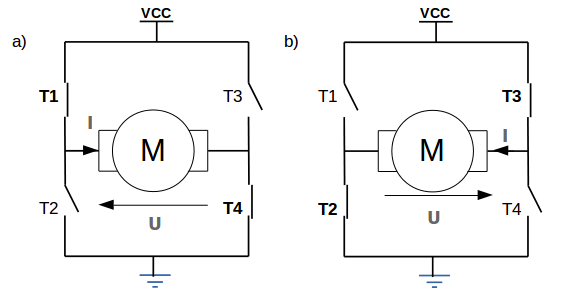
\includegraphics[width=0.5\textwidth]{images/MINE_Composants_PontH_Fonctionnement.png}
\end{center}


Il faut alors piloter en même temps deux des quatre transistors pour laisser passer du courant dans une direction particulière dans le moteur :

\begin{itemize}
	\item piloter T1 et T4 (figure a) permet de faire tourner le moteur dans un sens ;
	\item piloter T2 et T3 (figure b) permet de faire tourner le moteur dans l'autre sens.
\end{itemize}

\subsubsection{L293D ou SN754410NE}

Le composant \textbf{L293D} (ou son cousin \textbf{SN754410NE}) intègre deux structures de ce type pour pouvoir piloter 2 moteurs indépendamment dans deux directions (ou 4 moteurs dans une direction).

\begin{center}
	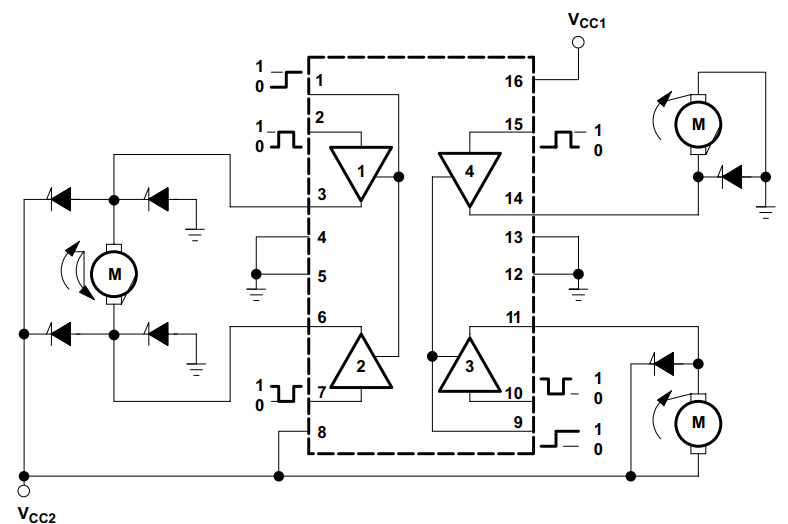
\includegraphics[width=0.6\textwidth]{images/L293D_TI.png}
	
	Schéma de cablage du L293D / Documentation Texas Instrument
\end{center}

Les \textbf{entrées 2 et 7} du composant permettent de faire \textbf{tourner le moteur dans un sens ou dans l'autre}. L'\textbf{entrée 1} est un \textbf{interrupteur général} des modules 1 et 2.

Les signaux des entrées 1, 2 et 7 sont des signaux de faible puissance provenant de la carte Nucléo. Les sorties 3 et 6 sont des sorties de puissance, qui tirent leur énergie de l'alimentation $V_{CC2}$. Une alimentation de faible puissance (typiquement 5V) - qui doit être indépendante de la source de puissance - doit également être fournie au composant sur $V_{CC1}$.

\subsection{Utilisation de signaux modulés en largeur d'impulsion}

Les \textbf{moteurs à courant continu} se pilotent grâce à des \textbf{tensions continues}. Or dans les deux structures vues précédemment, la tension appliquée au moteur ne peut prendre que 3 valeurs : $-V_{CC}$, $0V$ ou $V_{CC}$, ne laissant alors que 3 réactions possibles du moteur : tourner à une vitesse fixe $\Omega$ (dépendant de la valeur de $V_{CC}$) dans une direction ou dans une autre, ou être à l'arrêt.

\medskip

En utilisant le \textbf{principe de la modulation en largeur d'impulsions} (\textit{PWM} en anglais) de signaux numériques "rapides", il est toutefois possible de contrôler la vitesse de rotation des moteurs à courant continu. 

\begin{center}
	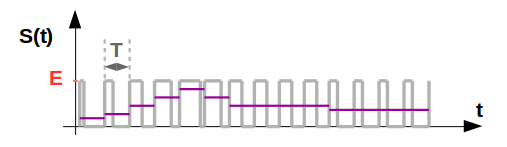
\includegraphics[width=0.6\textwidth]{images/MINE_ElecNum_PWM_Signal.png}
	
	Signal PWM et sa valeur moyenne
\end{center}


En effet, les systèmes mécaniques, que sont les moteurs, ont des \textbf{constantes de temps de réaction assez élevées} (de l'ordre de la centaine de millisecondes pour les moteurs de ce robot). En leur appliquant un signal rectangulaire suffisamment rapide, le moteur n'aura pas le temps de réagir aux fluctuations rapides du signal. Seul le \textbf{signal moyen} sera alors traduit par le moteur en consigne (système passe-bas).


\newpage
\subsection{Travail à réaliser}

\Manip Créer un nouveau projet dans \textbf{Keil Studio Cloud}, en vous basant sur l'exemple \textbf{\textsl{mbed-os-example-blinky-baremetal}} dans \textsc{Mbed OS 6}. 

\Manip Paramétrer les broches de commande du moteur de gauche en sortie modulée (\textsc{MOT\_L\_1} et \textsc{MOT\_L\_2}). Forcer le signal à un rapport cyclique de 0 dans la fonction d'initialisation.

\Manip Paramétrer la broche \textsc{MOT\_EN} en sortie standard. Forcer la sortie à 0 pour ce signal dans la fonction d'initialisation.

\Manip Ecrire une fonction qui permet de faire tourner le moteur gauche dans une direction à un rapport cyclique donné en argument (entre 0 et 100\%).

\Manip Ecrire une fonction qui permet de stopper le moteur.

\Manip Ecrire une boucle infinie qui permette de tester vos différentes fonctions :

\begin{itemize}
	\item lancer le moteur à 80\% pendant 2 secondes
	\item stopper le moteur pendant 3 secondes
	\item lancer le moteur à 50\% pendant 4 secondes
	\item stopper le moteur pendant 1 seconde
\end{itemize}

\Manip Connecter l'alimentation externe sur l'entrée d'alimentation du robot (connecteur J8 - voir partie \textbf{Alimentation électrique} de ce document).

\Manip Tester votre programme.


\noindent \rule{\linewidth}{1pt}

\textbf{Attention ! Couper l'alimentation externe lorsque vous n'utilisez pas le robot (en particulier lorsque vous modifier et téléverser votre programme dans la carte).}

\noindent \rule{\linewidth}{1pt}

\medskip

\Manip Faire le même travail pour le moteur droit.

\Manip Ajouter des fonctions permettant de faire avancer et reculer votre robot. Tester ces fonctions.


\newpage
%%%%%%%%%%%%%%%%%%%%%%%%%%%%%%%%%%%%%%%%%%%%%%%%
%%%%%%%%%%%%%    Etape 8
\section{Etape 8 / Acquérir des données des capteurs de ligne}

Les \textbf{capteurs de ligne} utilisés sur cette plateforme sont des \textbf{capteurs optiques}. Une \textbf{LED infrarouge} émet un signal vers le bas du robot qui est ensuite réfléchie plus ou moins fortement par le matériau présent au sol. Cette réflexion est alors captée par une \textbf{photodiode} ou un phototransistor.

\begin{center}
	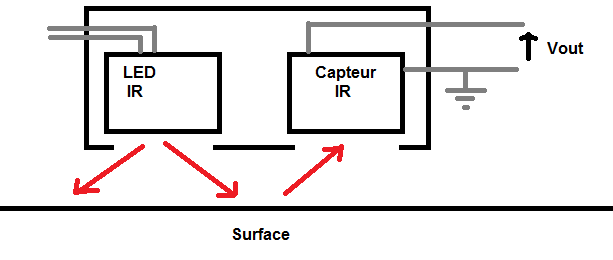
\includegraphics[width=0.6\textwidth]{images/capteur_ligne_gedgayblog.png}
	
	Principe du capteur de ligne / gedgeyblog.wordpress.com
\end{center}

Un comparateur est ensuite ajouté en sortie pour transmettre uniquement un signal numérique : '0' si ligne détectée, '1' sinon (ou inversement selon le type de compareteur utilisé). Un potentiomètre de réglage du seuil de détection est présent sur les capteurs. Une LED visible est également présente permettant de visualiser l'état du capteur (cela permet notamment de régler le seuil plus facilement).

\subsection{Travail à réaliser}

\Manip Créer un nouveau projet dans \textbf{Keil Studio Cloud}, en vous basant sur l'exemple \textbf{\textsl{mbed-os-example-blinky-baremetal}} dans \textsc{Mbed OS 6}.

\Manip Paramétrer les broches des \textbf{capteurs de ligne} en entrée d'interruption (\textsc{Line\_L}, \textsc{Line\_C} et \textsc{Line\_R}).

\Manip Ajouter une fonction d'interruption, exécutée lors de l'activation d'un des capteurs de ligne, permettant de stocker l'état des 3 capteurs dans 3 variables indépendantes (booléennes par exemple) et d'afficher leur valeur sur la console.

\Manip Tester votre programme à l'aide d'une feuille blanche contenant une ligne noire de largeur 2 à 3 cm.

\newpage
%%%%%%%%%%%%%%%%%%%%%%%%%%%%%%%%%%%%%%%%%%%%%%%%
%%%%%%%%%%%%%    Etape 9
\section{Etape 9 / Piloter les phares du robot}

Les phares du robot utilisent des LED trichromes "intelligentes" de type \textbf{WS2812}. Ces LEDs peuvent être mises en cascade et se pilotent à l'aide d'une trame numérique. Chaque LED nécessite 24 bits de données (8 bits par couleur - R/G/B).

\begin{center}
	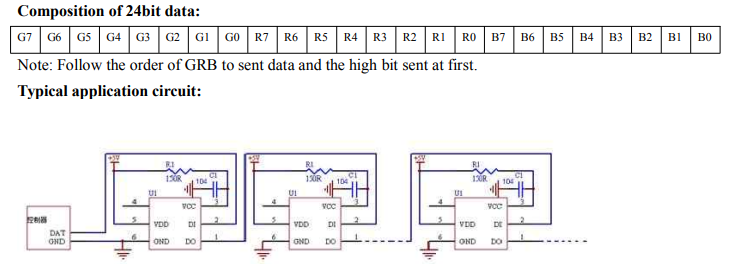
\includegraphics[width=0.9\textwidth]{images/W2812.png}
	
	Données et cablage WS2812 / Documentation Adafruit
\end{center}


\subsection{Bibliothèques }

Pour piloter ce type de LED, le LEnsE a modifié deux bibliothèques disponibles dans le fichier \textsl{example\_WS2812.zip} :

\begin{itemize}
	\item \textbf{PixelArray} : permettant de créer des tableaux de pixels R,V,B (rouge, vert et bleu) ;
	\item \textbf{WS2812} : permettant de transmettre les données aux LEDs de type WS2812.
\end{itemize}

Ce fichier est disponible sur le site du LEnsE dans la rubrique \textit{Année / Première Année / Interfaçage Numérique S6 / Bloc 1 Systèmes embarqués / Robotique / Exemples MBED pour STM32}.

\subsubsection{Importation des bibliothèques}

\Manip Décompresser le fichier archivé dans un répertoire de votre espace personnel.

Il contient 5 fichiers dont les 4 fichiers des bibliothèques mentionnées précédemment (un fichier .h et un fichier .cpp par bibliothèque).

\Manip Créer un nouveau projet dans \textbf{Keil Studio Cloud}, en vous basant sur l'exemple \textbf{\textsl{mbed-os-example-blinky-baremetal}} dans \textsc{Mbed OS 6}. 

\bigskip

Vous devez importer les deux bibliothèques dans votre projet de la manière suivante :

\begin{enumerate}
	\item Créer un répertoire \textsl{\textbf{Libs}} dans votre projet \textbf{Keil Studio Cloud}
	\item Déplacer les fichiers \textsl{PixelArray.h}, \textsl{PixelArray.cpp}, \textsl{WS2812.h} et \textsl{WS2812.cpp} dans ce répertoire.
\end{enumerate}

\newpage
\subsection{Travail à réaliser}

On se propose de tester le code \textsl{neoled\_control.cpp}. Ce fichier est disponible sur le site du LEnsE dans la rubrique \textit{Année / Première Année / Interfaçage Numérique S6 / Bloc 1 Systèmes embarqués / Robotique / Exemples MBED pour STM32}.

\Manip Tester le code fourni, en ayant au préalable importer les deux bibliothèques précédentes dans votre projet.

\Manip Modifier la couleur des deux LEDs présentes sur ce phare.

\Manip Ajouter la configuration des 3 autres phares.

\Manip Créer une fonction qui permet d'allumer les phares avant, une autre fonction qui permet d'allumer les phares arrière.

\Manip Tester vos différentes fonctions.


\newpage
\strut % empty page
%%%%%%%%%%%%%%%%%%%%%%%%%%%%%%%%%%%%%%%%%%%%%%%%
%%%%%%%%%%%%%    Séances 3 et 4 détaillées
\begin{minipage}[c]{.25\linewidth}
	
\includegraphics[width=4cm]{images/Logo-LEnsE.png}
\end{minipage} \hfill
\begin{minipage}[c]{.4\linewidth}

\begin{center}
\vspace{0.3cm}
{\Large \textsc{Interfaçage Numérique}}

\medskip

6N-047-SCI \qquad \textbf{\Large Bloc Robot}

\end{center}
\end{minipage}\hfill

\vspace{0.5cm}

\noindent \rule{\linewidth}{1pt}

{\noindent\Large \rule[-7pt]{0pt}{30pt} \textbf{Séances 3 et 4} / Robot suiveur de ligne autonome} 

\noindent \rule{\linewidth}{1pt}

Les deux séances suivantes seront consacrées au pilotage du robot pour lui permettre de suivre une ligne ou/et d'éviter les obstacles qu'il rencontre sur son chemin.

%%%%%%%%%%%%%%%%%%%%%%%%%%%%%%%%%%%%%%%%%%%%%%%%
%%%%%%%%%%%%%    Etape 10
\section{Etape 10 / Définir et tester une première structure de code}

On souhaite à présent réaliser le \textbf{programme principal} du robot lui permettant de \textbf{se déplacer de manière autonome} en suivant une ligne.


\subsection{Travail à réaliser}

\Manip En vous basant sur les différentes fonctions que vous avez écrites précédemment (avancer, reculer, tourner...) et des valeurs des différents capteurs de ligne, réaliser le programme permettant au robot de suivre une ligne.

\Manip Tester la robustesse de votre application sur un parcours plus grand.

%%%%%%%%%%%%%%%%%%%%%%%%%%%%%%%%%%%%%%%%%%%%%%%%
%%%%%%%%%%%%%    Etape 11
\section{Etape 11 / Acquérir les signaux du capteur ultrason}

La maquette est équipée d'un capteur de distance à ultrasons. Le principe est décrit dans le schéma suivant :

\begin{center}
	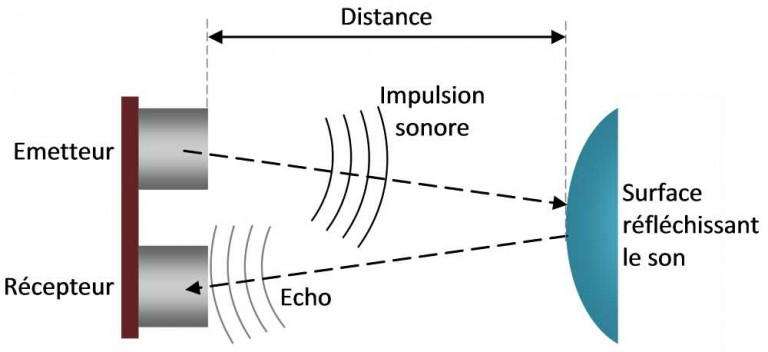
\includegraphics[width=0.5\textwidth]{images/Principe_Ultrasons_1_arduino.blaisepascal.fr.jpg}
	
	Principe du capteur de distance à ultrasons / https://arduino.blaisepascal.fr/capteur-de-distance-a-ultrasons/
\end{center}

Un \textbf{émetteur} génère une \textbf{impulsion sonore brève} (à une fréquence non audible). Cette onde est \textbf{réfléchie} par la surface à détecter. L'onde retour, appelée \textsl{écho} est reçue par un \textbf{récepteur}. On mesure alors le \textbf{temps} entre le moment où l'onde est émise et le moment où l'écho revient - souvent nommé temps de vol. Ces ondes se propageant à la vitesse du son (environ 340m/s), il est alors possible de revenir sur la distance parcourue par cette onde.

\newpage
\subsection{Travail à réaliser}

On se propose de tester le code \textsl{dist\_us.cpp}. Ce fichier est disponible sur le site du LEnsE dans la rubrique \textit{Année / Première Année / Interfaçage Numérique S6 / Bloc 1 Systèmes embarqués / Robotique / Exemples MBED pour STM32}.

\Manip Tester ce code et afficher sur la console Série la durée obtenue en  plaçant un objet "plat" devant le robot. Recommencer l'expérience en faisant varier la distance entre l'objet et le robot.

\Manip Visualiser les signaux des broches D4 et D3 à l'aide de l'oscilloscope.

\Quest Quelle est la limite de détection de ce capteur ?

\newpage
%%%%%%%%%%%%%%%%%%%%%%%%%%%%%%%%%%%%%%%%%%%%%%%%
%%%%%%%%%%%%%    Etape 12
\section{Etape 12 / Piloter le servomoteur associé au capteur ultrason}

Un servomoteur est un actionneur qui réalise une rotation d'un angle calibré en fonction d'une commande externe.

\begin{center}
	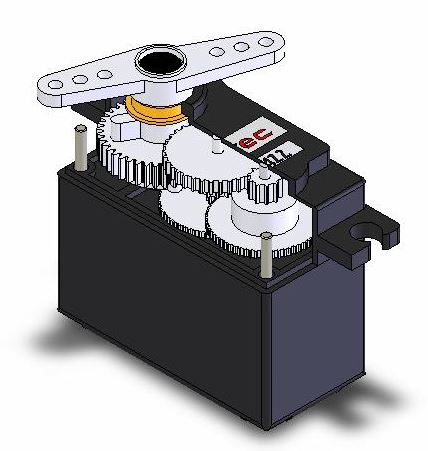
\includegraphics[width=0.3\textwidth]{images/MINE_Nucleo_servomoteur-redohm.jpg}
	
	Servomoteur - coupe interne (Crédit : redohm.fr)
\end{center}

Le pilotage d'un servomoteur se fait à l'aide d'un \textbf{signal modulé en largeur d'impulsions}. Le signal de commande est un \textbf{signal rectangulaire} (numérique) de période fixée à 20 ms. C'est ensuite la durée du temps haut qui permet de modifier l'angle de sortie du servomoteur :

\begin{center}
	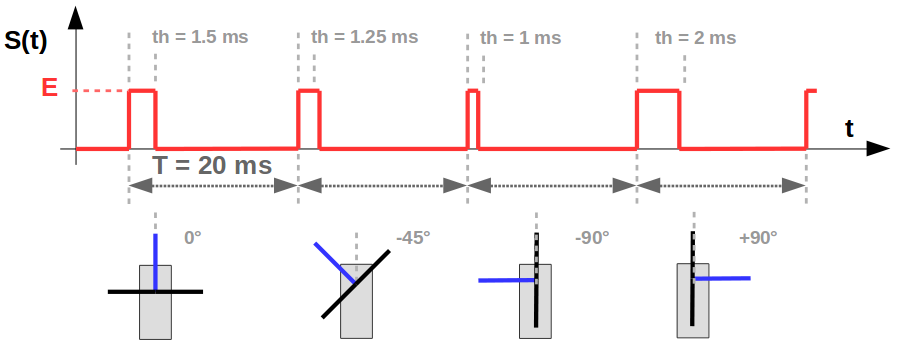
\includegraphics[width=0.8\textwidth]{images/MINE_Nucleo_servomoteur.png}
\end{center}

\subsection{Travail à réaliser}

On se propose de tester le code \textsl{pwm\_servo.cpp}. Ce fichier est disponible sur le site du LEnsE dans la rubrique \textit{Année / Première Année / Interfaçage Numérique S6 / Bloc 1 Systèmes embarqués / Exemples MBED pour STM32}.

\Manip Tester le code fourni. 

\Manip Créer une fonction permettant de positionner le servomoteur à un angle particulier. Tester votre fonction. 



\newpage
\strut % empty page
%%%%%%%%%%%%%%%%%%%%%%%%%%%%%%%%%%%%%%%%%%%%%%%%
%%%%%%%%%%%%%    Autres possibilités
\begin{minipage}[c]{.25\linewidth}
	
\includegraphics[width=4cm]{images/Logo-LEnsE.png}
\end{minipage} \hfill
\begin{minipage}[c]{.4\linewidth}

\begin{center}
\vspace{0.3cm}
{\Large \textsc{Interfaçage Numérique}}

\medskip

6N-047-SCI \qquad \textbf{\Large Bloc Robot}

\end{center}
\end{minipage}\hfill

\vspace{0.5cm}

\noindent \rule{\linewidth}{1pt}

{\noindent\Large \rule[-7pt]{0pt}{30pt} Autres fonctionnalités} 

\noindent \rule{\linewidth}{1pt}


\section{Acquérir des données de l'accéléromètre (I2C)}

Le composant présent sur le robot est un \textbf{accéléromètre et magnétomètre} intégrés sur une même puce de silicium. Sa référence est \textbf{FXOS8700CQ}. Ce composant est intégré au module \textit{MikroE} \textbf{DOF6 - IMU Click}.

\subsection{Brochage}

Ce module fonctionne à l'aide du protocole I2C.

\begin{center}
\begin{tabular}{|l|l|l|l|}
\hline 
Maquette & \textbf{Broche Nucléo} & Type & Description \\ 
\hline 
\textsc{SDA} & PB9 & Entrée-Sortie & Signal de données bidirectionnel \\ 
\textit{SCL} & PB8 & Sortie & Signal d'horloge\\
\hline 
\textsc{Reset} & PC4 & Sortie & Reset matériel du composant\\ 
\textit{Interrupt} & PB10 & Entrée & Interruption sur réception\\ 
\hline 
\end{tabular} 
\end{center}


\subsection{Protocole I2C}

DESCRIPTION PROTOCOLE et CONNECTIQUES !

\bigskip

\textsc{Attention !} Les broches utilisées sur la carte Nucléo pour l'I2C ne sont pas celles par défaut. Il est indispensable de préciser les broches SDA et SCL à l'aide des méthodes suivantes :

\begin{lstlisting}
Wire.setSDA( PB9 );    
Wire.setSCL( PB8 ); 
\end{lstlisting}

\bigskip

\Manip Ouvrir le code \textsl{09\_accelero.ino} fourni. Compiler ce code et téléverser ce code dans la carte Nucléo.

Ce code contient les fonctions \textsl{test\_FXOS()} et \textsl{read\_i2c\_buffer()}, ainsi que des définitions des registres internes du composant.

\Manip 

\subsection{Configuration}


\subsection{Récupération des données}

\textit{These registers contain the X-axis, Y-axis, and Z-axis 14-bit left-justified sample data expressed as 2's complement numbers.} [NXP Doc p.52 of 113] 


\section{Autres fonctionnalités de la carte}

La carte de contrôle est également équipée de 2 connecteurs permettant d'accueillir :

\begin{itemize}
	\item un \textbf{accéléromètre} MikroE-6DOF IMU 3 Click ;
	\item un module de \textbf{communication} nRF24L01 ;
\end{itemize}

Elle est également équipée de \textbf{deux capteurs de température} :
\begin{itemize}
	\item un capteur analogique - MCP9700
	\item un capteur à sortie numérique - TC74A2
\end{itemize}


\subsubsection{Capteur température numérique / TC74A2}

Ce module fonctionne à l'aide du protocole I2C.

\begin{center}
\begin{tabular}{|l|l|l|l|}
\hline 
Maquette & \textbf{Broche Nucléo} & Type & Description \\ 
\hline 
\textsc{SDA} & PB9 & Entrée-Sortie & Signal de données bidirectionnel \\ 
\textit{SCL} & PB8 & Sortie & Signal d'horloge\\
\hline 
\end{tabular} 
\end{center}


\subsubsection{Communication nRF24L01}

Ce module fonctionne selon le protocole SPI. \textit{Il doit nécessairement être utilisé avec un second module afin de pouvoir transmettre des données entre deux microcontroleurs.}

\begin{center}
\begin{tabular}{|l|l|l|l|}
\hline 
Maquette & \textbf{Broche Nucléo} & Type & Description \\ 
\hline 
\textsc{SPI} & & & \\ 
\textit{SCK} & PC10 & Sortie & Signal d'horloge\\
\textit{MISO} & PC11 & Entrée & Données entrantes\\
\textit{MOSI} & PC12 & Sortie & Données sortantes\\ 
\hline  
\textit{CS} & PA14 & Sortie & Sélection du composant\\ 
\textit{CE} & PD2 & Sortie & Validation du composant (puissance)\\ 
\textit{INT} & PA15 & Entrée & Interruption sur réception\\ 
\hline  
\end{tabular} 
\end{center}


\subsubsection{Utilisation de la sortie modulée PB7}
	
\begin{lstlisting}
LL_GPIO_SetAFPin_0_7(GPIOB,  GPIO_PIN_7,  GPIO_AF1_TIM2);
\end{lstlisting}


\subsection{Traceur Série}

\begin{lstlisting}
  Serial.print(valeur1);
  Serial.print(",");
  Serial.print(valeur2);
  Serial.print(",");
  Serial.print(valeur3);
  Serial.print(",");
  Serial.print(valeur4);
  Serial.println();
\end{lstlisting}


%%%%%%%%%%%%%%%%%%%%%%%%%%%%%%%%%%%%%%%%%%%%%%%%
%%% RESSOURCES COMPLEMENTAIRES		

\newpage
% Ressources
\begin{center}
	\begin{minipage}{2.5cm}
	\begin{center}
		
\includegraphics[width=5cm]{images/Logo-LEnsE.png}
	\end{center}
\end{minipage}\hfill
\begin{minipage}{10cm}
	\begin{center}
	\textbf{Institut d'Optique Graduate School }\\[0.1cm]
    \textbf{Interfaçage Numérique}


	\end{center}
\end{minipage}\hfill


\vspace{2cm}


{\Large \bfseries \textsc{Interfaçage Numérique}} \\[0.5cm]
{\large \bfseries Travaux Pratiques} \\[0.2cm]
Semestre 6

\vspace{1cm}

% Title
\rule{\linewidth}{0.4mm} \\[0.4cm]
{ \Large \bfseries\color{violet_iogs} Ressources \\[0.4cm] }
\rule{\linewidth}{0.4mm} \\[1cm]
{\large Bloc Robot}

\end{center}

\vspace{3cm}

\textbf{\large Liste des ressources}
\begin{itemize}
	\item \hyperref[doc:robot_schematic]{Schéma de la carte du robot Joy-It Car}
	\item \hyperref[doc:robot_pcb]{PCB de la carte du robot Joy-It Car}
\end{itemize}

\vfill

\newpage
\strut % empty page
% Ressources
\titleformat{\section}
  {\null}{}{0pt}{}


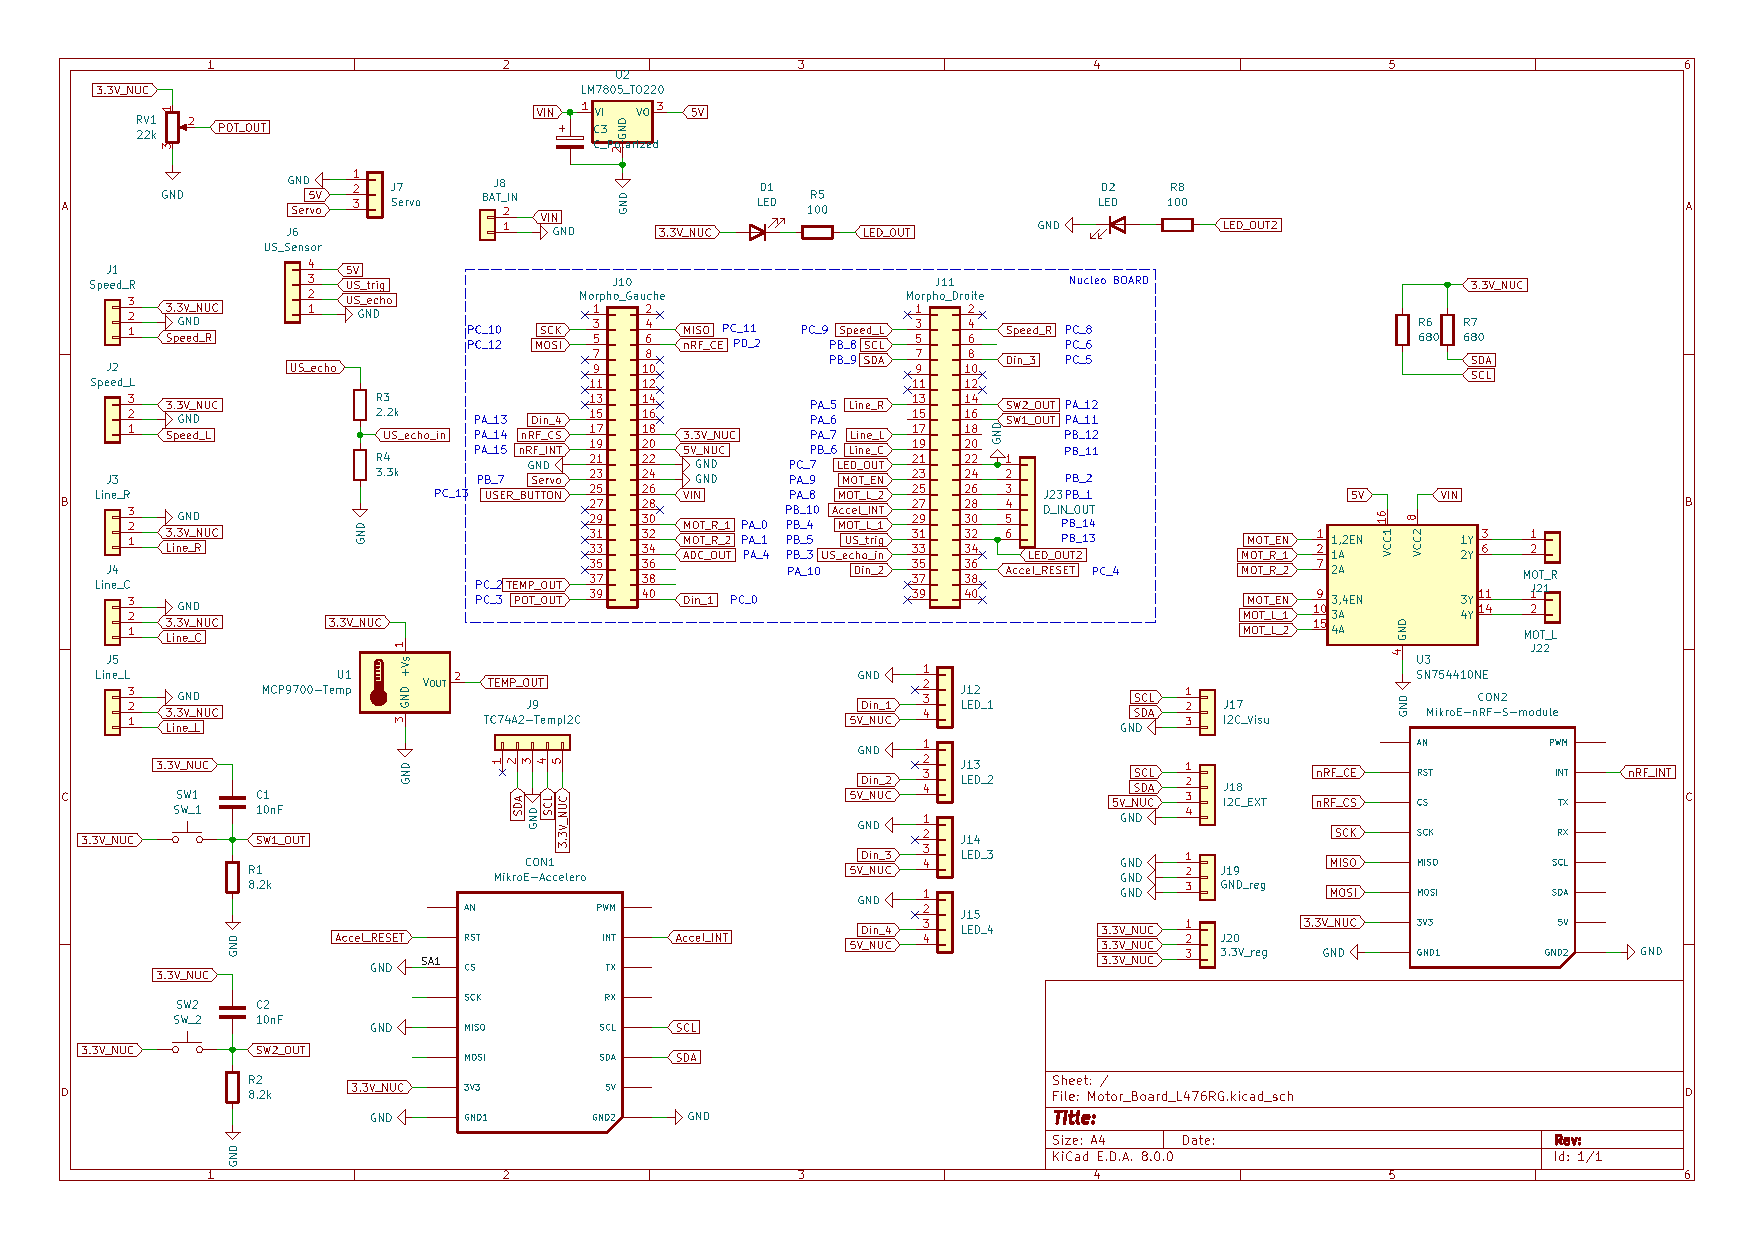
\includepdf[pages=1, landscape=true, pagecommand={\section{\texorpdfstring{\hspace{-1em}}{Schéma Robot}}}\label{doc:robot_schematic}]{ressources/Motor_Board_L476RG_sch.pdf}


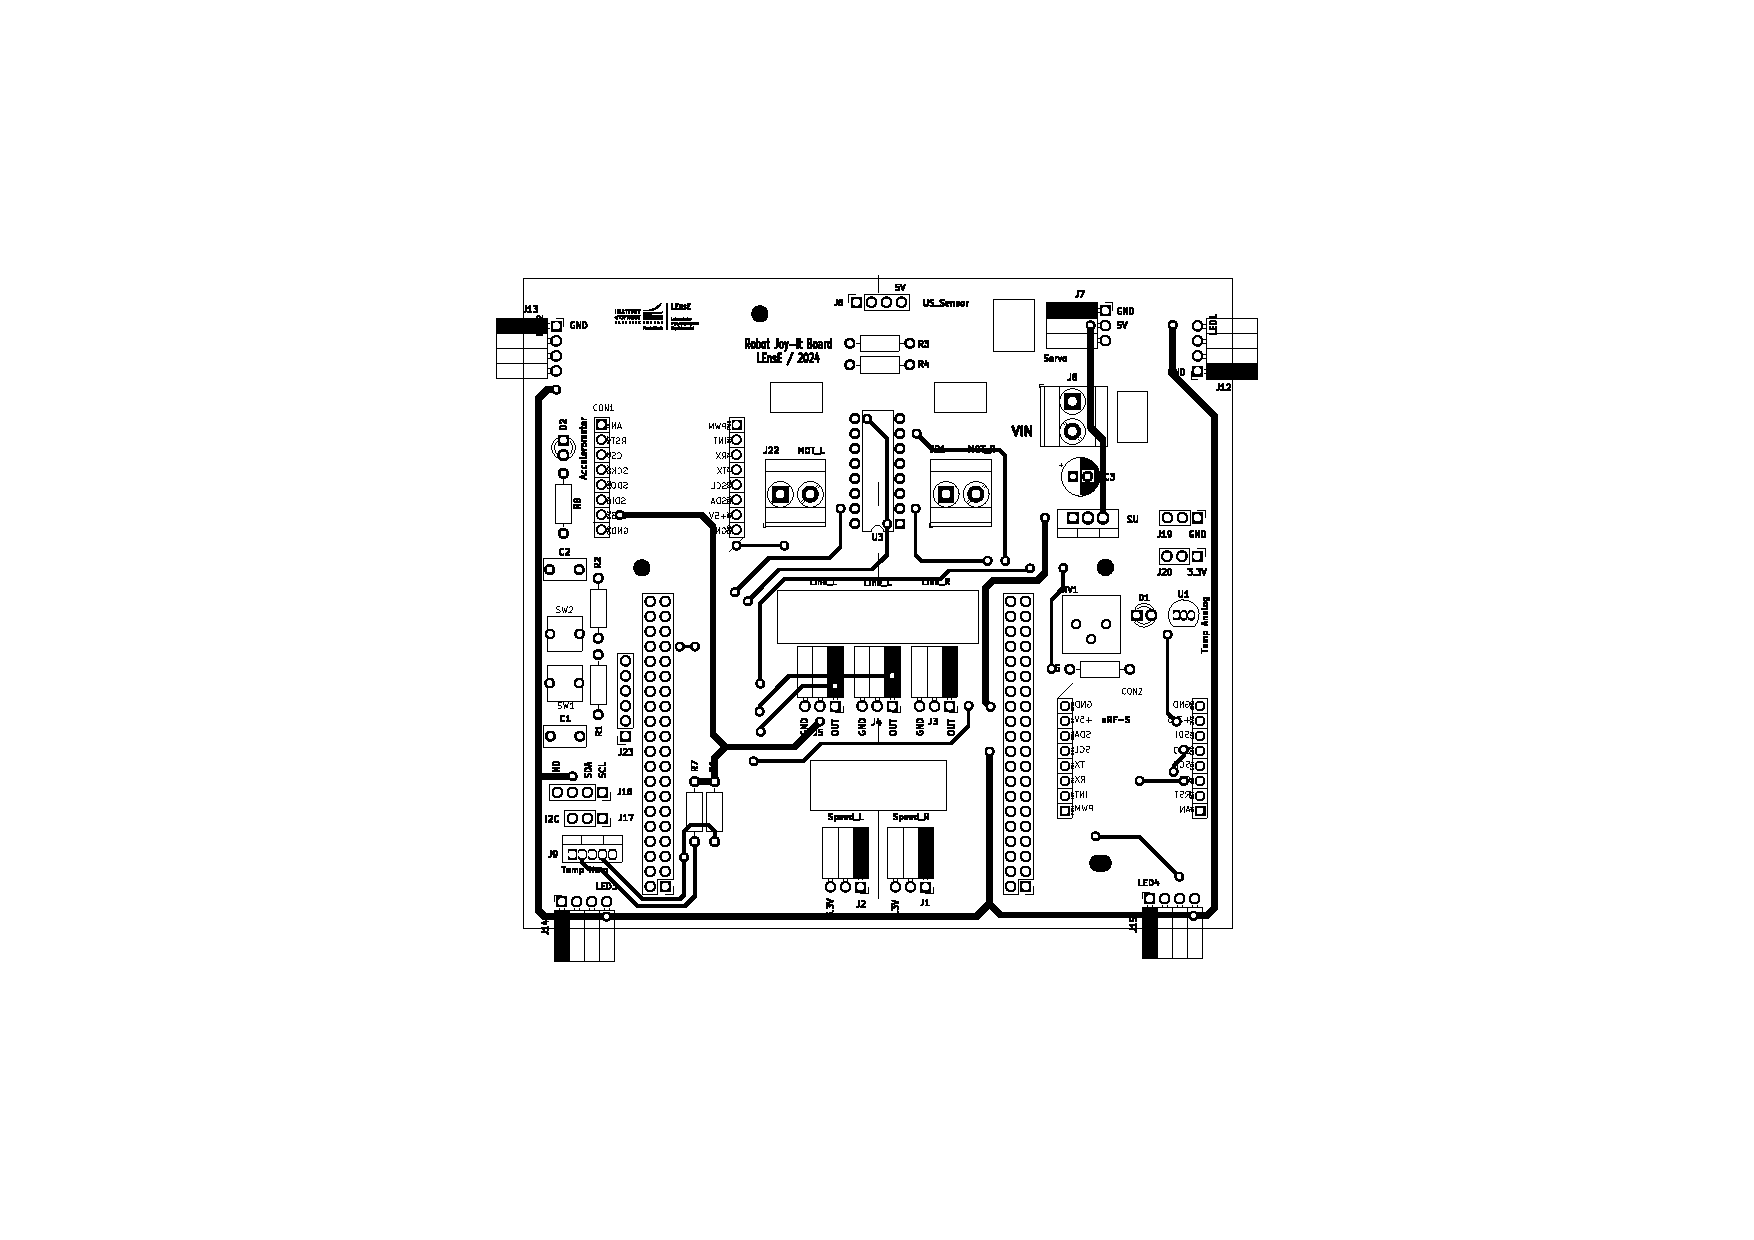
\includepdf[pages=1, landscape=true, pagecommand={\section{\texorpdfstring{\hspace{-1em}}{PCB Robot}}}\label{doc:robot_pcb}]{ressources/Motor_Board_L476RG_pcb.pdf}


\end{document}


